%-------------------------------------------------------------------------------
%	PAQUETES Y OTRAS CONFIGURACIONES
%-------------------------------------------------------------------------------
%-------------------------------------------------------------------------------
%	PAQUETES Y OTRAS CONFIGURACIONES
%-------------------------------------------------------------------------------
\documentclass{tufte-handout}
%\documentclass[paper=letter, fontsize=11pt]{scrartcl} % Tamaño de papel y letra para el documento
\usepackage{geometry}
\geometry{left=1.2cm, right=6.2cm, top=2.5cm, bottom=2.5cm}
\usepackage{color}
\usepackage[utf8]{inputenc} % Los caracteres acentuados se pueden escribir normalmente en el código
\usepackage[T1]{fontenc} % Configuración de fuente de salida
\usepackage{cmbright}
\usepackage[sfdefault]{noto}
\usepackage[T1]{fontenc}
\normalfont
\usepackage{graphicx} % Paquetes para incluir imágenes
\usepackage{multicol}
\usepackage{circuitikz}
\usepackage{tikz}
\usetikzlibrary{arrows}

\usepackage{sectsty} % Paquete para configuración de secciones
\allsectionsfont{\centering \normalfont \scshape} % Los títulos de las secciones son centrados, con la misma fuente y pequeñas mayúsculas

\usepackage{todonotes}
\usepackage{microtype}
\renewcommand{\figurename}{Figura}

\usepackage{listings}
\renewcommand{\lstlistingname}{Código}
\lstdefinestyle{mystyle}{
    basicstyle=\footnotesize,
    breakatwhitespace=false,
    breaklines=true,
    captionpos=b,
    keepspaces=true,
    numbers=left,
    numbersep=5pt,
    showspaces=false,
    showstringspaces=false,
    showtabs=false,
    tabsize=2
}
\lstset{style=mystyle}

% \usepackage{fancyhdr} % Paquete para personalizar pies y cabeceras de página
% \pagestyle{fancyplain} % Todas las páginas con las mismas cabeceras y pies de página
% \fancyhead{} % Sin cabecera
% \fancyfoot[L]{} % Vacío en la izquierda del pie de página
% \fancyfoot[C]{} % Vacío en el centro del pie de página
% \fancyfoot[R]{\thepage} % Número de página en el pie de pagina
% \renewcommand{\headrulewidth}{0pt} % Sin lineas en la cabecera
% \renewcommand{\footrulewidth}{0pt} % Sin lineas en el pie de página
% \setlength{\headheight}{13.6pt} % Altura de cabecera
%
% \numberwithin{equation}{section} % Numera ecuaciones en cada sección
% \numberwithin{figure}{section} % Numera figuras en cada sección
% \numberwithin{table}{section} % Numera tablas en cada sección
%
% \setlength\parindent{0pt} % Quita la indentación de los párrafos

\newcommand{\horrule}[1]{\rule{\linewidth}{#1}} % Comando personalizado para hacer linea horizontal

%-------------------------------------------------------------------------------
%	TITULO
%-------------------------------------------------------------------------------
\title{Práctica 5 - Control de servomotores\\Interfaces y periféricos para robots}
\author{Roberto Cadena Vega} % Nombre del profesor
\date{}
%-------------------------------------------------------------------------------
%	EMPIEZA EL DOCUMENTO
%-------------------------------------------------------------------------------
\begin{document}
\maketitle % Imprime el título
%-------------------------------------------------------------------------------
%	OBJETIVOS
%-------------------------------------------------------------------------------
\section{Objetivos}

	Controlar la posición de un motor de corriente directa con un sensor de realimentación (servomotor).
%-------------------------------------------------------------------------------
%	CONOCIMIENTOS PREVIOS
%-------------------------------------------------------------------------------
\section{Conocimientos Previos}
%-------------------------------------------------------------------------------
	\subsection{Controladores}

		\begin{marginfigure}
			\begin{center}
				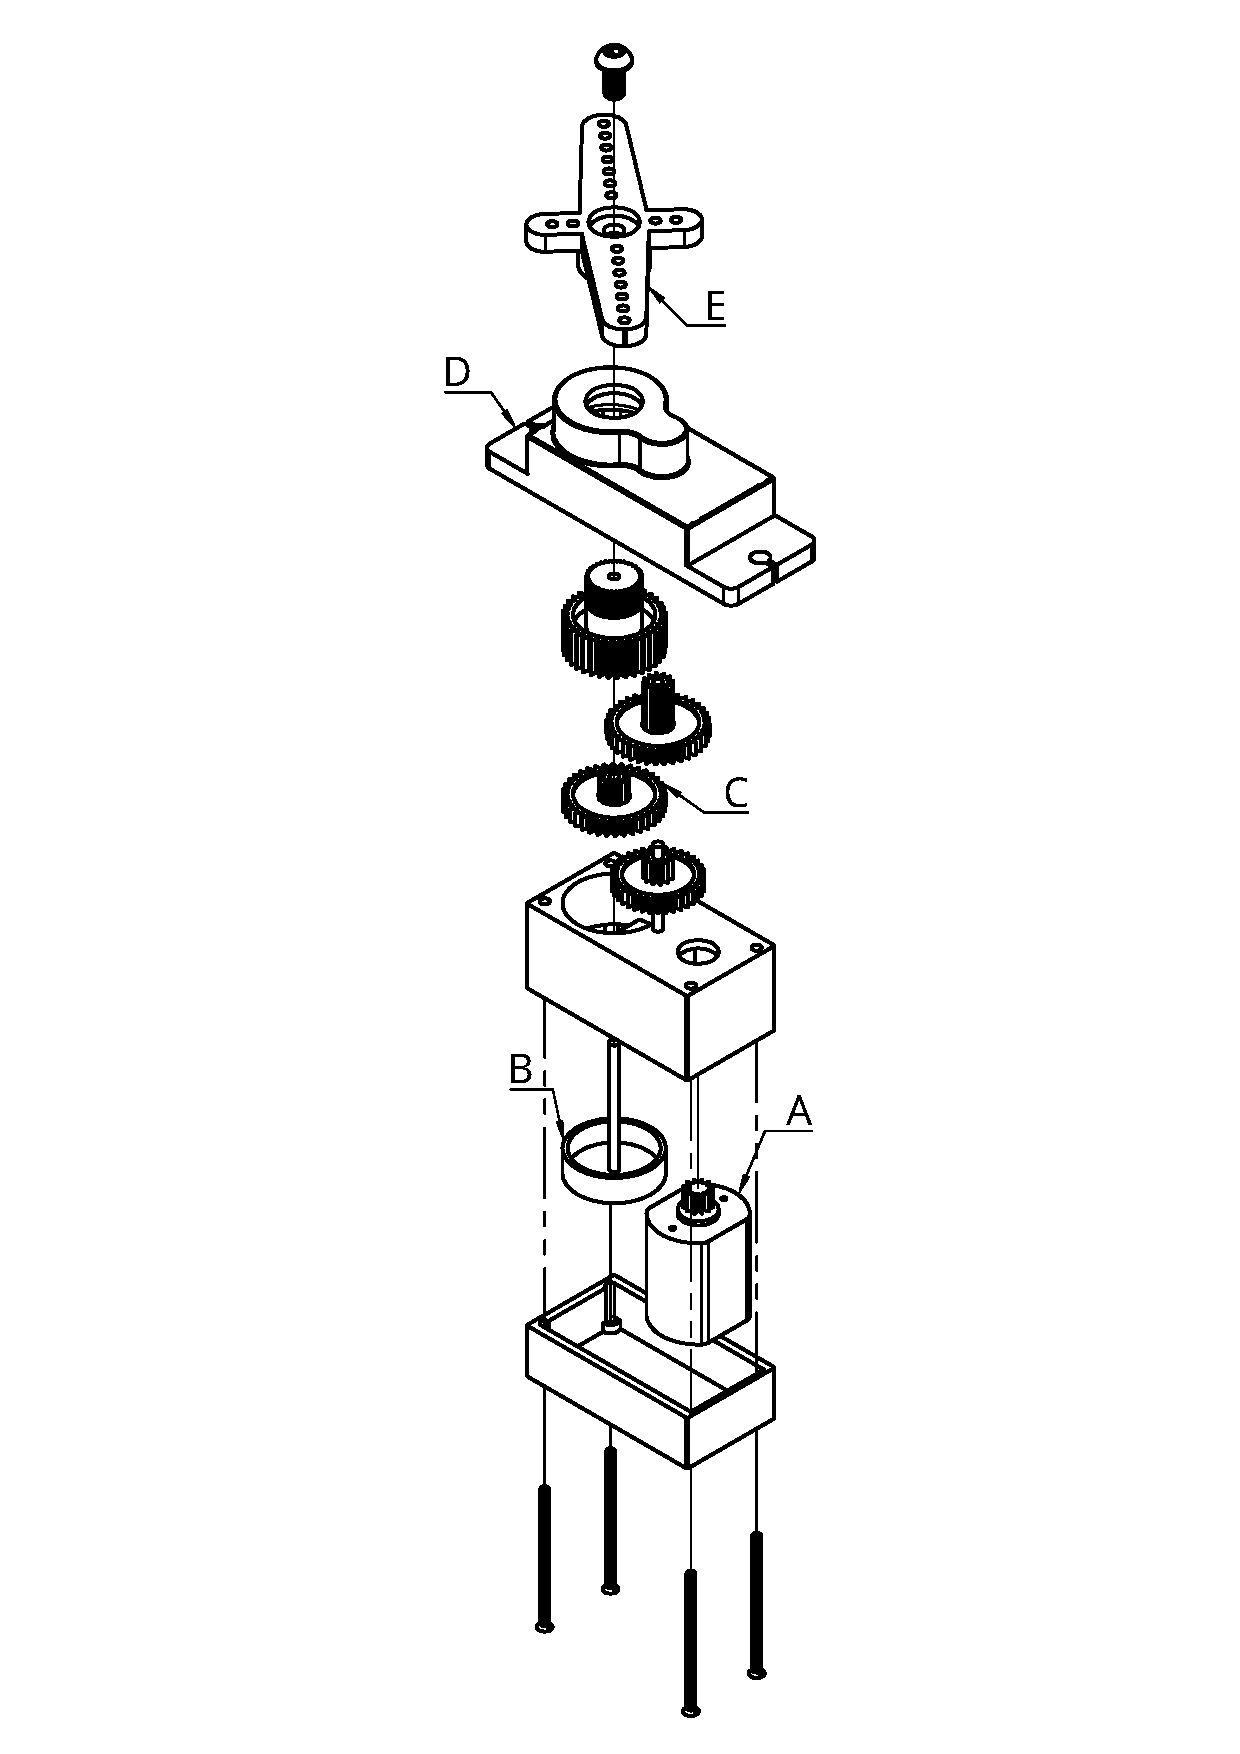
\includegraphics[width=0.6\textwidth]{images/servo.pdf}
				\caption{Explosion de un servomotor comercial}
				\label{fig:servomotor}
			\end{center}
		\end{marginfigure}

		En esta práctica utilizaremos primero el servomotor, como el de la figura \ref{fig:servomotor}, de la manera en que el fabricante esperaba que lo usaramos, despues lo modificaremos de tal manera en que podamos controlarlo completamente desde el Arduino.

		En primer lugar debemos saber como funciona normalmente; para esto lo conectaremos de acuerdo a las instrucciones del fabricante, tomando cuidado de conectar el cable de señal al pin 13 de la tarjeta de desarrollo Arduino, para darle la señal de control por medio de este.

		Ahora podemos subir el siguiente código a nuestro Arduino, con el que podremos modificar su posición por medio de comandos en el monitor serial del IDE de Arduino.

		\begin{multicols}{2}
			\lstinputlisting[language=C]{codigos/servo_comercial_serial.ino}
		\end{multicols}

		En este código, la estructura general es que intentará recibir datos del puerto serial, y después mandará la señal al servomotor. Cuando recibe datos del puerto serial supondrá que es un número entre $0^o$ y $180^o$ y hará el cálculo de los retardos necesarios para dar la señal correcta al servomotor. Si analizamos este cálculo, podremos ver que cuando la posición es $0^o$, el tiempo que la señal permanecerá encendida es $0.9ms$ y el tiempo que permanecerá apagada es $2.1ms + 17ms = 19.1ms$, es decir, una señal de $20ms$ en total; cuando la posición es $180^o$, el tiempo de encendido es $2.1ms$, el tiempo de apagado es $0.9ms + 17ms = 17.9ms$, es decir, una señal de $20ms$ en total.

		\tikzset{timing/intext/.append style={timing/draw grid}}
		\tikzset{timing/grid/.append style={step=1}}
		\tikzset{timing/grid/.append style={shift={(0.1,0)}}}
		\tikzset{timing/grid/.append style={ultra thin}}
		%\tikztimingsetwscale{2\wscale}
		\begin{center}
			\begin{tabular}{l l}
				$S_{0^o}$ & \texttiming[xscale=1.5,very thick]{0.1L 0.9H 19.1L 0.1L} \\
				$S_{30^o}$ & \texttiming[xscale=1.5,very thick]{0.1L 1.1H 18.9L 0.1L} \\
				$S_{90^o}$ & \texttiming[xscale=1.5,very thick]{0.1L 1.5H 18.5L 0.1L} \\
				$S_{180^o}$ & \texttiming[xscale=1.5,very thick]{0.1L 2.1H 17.9L 0.1L} \\
			\end{tabular}
		\end{center}

		Cabe añadir que si esta señal dura $20ms$ en su totalidad, se tiene que enviar cada $20ms$, dependiendo de cada fabricante, es posible que el servomotor mantenga esta posición hasta que llegue una señal nueva, o bien, que si no llega una nueva señal despues de $20ms$, el controlador del servomotor suponga que el motor debe de ser apagado y el servomotor no conservará su posición al aplicarsele un par de torsión. Tambien es posible que el servomotor utilice un esquema diferente de excitación con tiempos diferentes a los establecidos en este código, en este caso será necesario modificar estos tiempos para adecuarse a la información del datasheet del servomotor.

		En este punto deberás llenar la primer tabla de la hoja de anotaciones, con los tiempos que le toma a tu servomotor moverse de la posición $0^o$ a la posición $180^o$ o de la posición $180^o$ a la posición $0^o$, para obtener un tiempo promedio de la operación realizada por el servomotor.

		\subsection{Trayectorias dependientes del tiempo}

		Si ahora queremos medir el error que va a tener este servomotor en una cierta trayectoria, necesitamos cargar el siguiente código el cual dará una señal senoidal al servomotor con una frecuencia variable:

		\begin{fullwidth}
			\begin{multicols}{2}
				\lstinputlisting[language=C]{codigos/servo_comercial_serial_senoidal_variable.ino}
			\end{multicols}
		\end{fullwidth}

		Este código empezará dando una señal senoidal al servomotor, haciendo que se mueva de $0^o$ hasta $180^o$ y de regreso, con una frecuencia de $1Hz$ para empezar, y con la posibilidad de enviar la frecuencia requerida por medio del monitor serial. Este código reutiliza elementos del pasado, pero antes de definir la posición a la que se debe mover el servomotor, primero calcula la posición por medio de una función senoidal que depende del tiempo que el Arduino ha permanecido encendido.

		Si jugamos con este código, enviando valores por medio del puerto serial, podremos notar que mientras mayor sea la frecuencia de la señal senoidal, menor es el angulo que el servomotor esta recorriendo, no puede moverse lo suficientemente rápido antes de que tenga que regresar de nuevo.

		En este punto deberás llenar la segunda tabla con el angulo que recorre el servomotor dependiendo de la frecuencia dada.

		\subsection{Hacking}

		\textbf{¡Peligro!} - A partir de este punto se harán modificaciones importantes al servomotor las cuales harán dificil el volver a resolver los puntos anteriores, por lo que es importante que hayas terminado las primeras dos tablas y hayas validado tu trabajo con el profesor, antes de empezar a trabajar en esta sección de la práctica.

		Una vez que hemos caracterizado el desempeño de nuestro servomotor, podemos seguir adelante con el diseño de un controlador por medio de la tarjeta de desarrollo Arduino, para esto necesitaremos abrir la parte inferior del servomotor: debes tener cuidado con no abrir el compartimiento de la transmisión de engranes, o bien tratarlos con el suficiente cuidado. Como se ve en la figura \ref{fig:servomotor}, la transmisión de engranes identificada con la etiqueta (C), esta acoplada al motor DC (A) y al potenciometro (B) a través de una carcasa plástica la cual esta fija con la tapa inferior y la tapa superior (D) por medio de tornillos, estos deben ser removidos para acceder a las conexiones en la tapa inferior, pero a su vez pueden aflojar la conexion de la tapa superior; mas aún si la transmisión es desarmada, es facil volver a armarla, pero comúnmente estara cubierta de grasa de litio (sustancia blanca y viscosa), por lo que te mancharas las manos y probablemente la ropa si es que no tienes cuidado. Muchas veces ayuda comectar el eslabon de salida (E) a la tranmisión para evitar que la transmisión tenga juego y se desensamble en el proceso de abrir la tapa inferior del servomotor.

		Una vez que tengas el servomotor abierto deberás retirar el controlador actual, desoldando o cortando los cables que entran a este y añadiendo longitud a los cables, los cuales deben ser, dos conductores del motor CD y tres conductores del potenciometro. Una vez que estos cables han sido alargados, se puede cerrar el servomotor de nuevo.

		Los dos conductores del motor CD deben ser conectados al circuito de potencia adquirido (L293D o L298N), las señales de control para este circuito vendrán del Arduino y estaran marcadas como \texttt{m1} y \texttt{m2}. Los tres conductores del potenciometro serán conectados a $0V$, $5V$ y al pin marcado como \texttt{pot\_pin} en el código; de tal manera que el Arduino detecte un voltaje en este pin entre $0V$ y $5V$ dependiendo de la posición del servomotor.

		Esta parte de la práctica es tardada y delicada por lo que la recomendación general es que se haga en casa, con tiempo suficiente para corregir errores que pudieran suceder, previamente se deben tomar recomendaciones del profesor dependiendo del tipo de servomotor que se adquirió para esta práctica.
		\newpage

		Una vez con nuestro circuito conectado, es momento de probar el primer código:

		\begin{fullwidth}
			\begin{multicols}{2}
				\lstinputlisting[language=C]{codigos/servo_mod_control_p_serial.ino}
			\end{multicols}
		\end{fullwidth}

		Este código intentará recibir la referencia de la posición deseada del puerto serial, leerá la posición del potenciometro, mandará este dato por el puerto serial, calculará el error entre la posición deseada y la posición real, calculará la señal necesaria para mover el motor a la posición deseada, y por ultimo, ira hacia adelante o hacia atras, dependiendo de si la señal necesaria es positiva o negativa. Si dibujamos un diagrama de bloques de la secuencia de información se verá asi:

		\begin{center}
			\tikzstyle{block} = [draw, rectangle,
	    minimum height=3em, minimum width=6em]
			\tikzstyle{sum} = [draw, circle, node distance=1cm]
			\tikzstyle{input} = [coordinate]
			\tikzstyle{output} = [coordinate]
			\tikzstyle{pinstyle} = [pin edge={to-,thin,black}]

			\begin{tikzpicture}[auto, node distance=2cm,>=latex']
			    \node [input, name=input] {};
			    \node [sum, right of=input] (sum) {};
			    \node [block, right of=sum] (controller) {Control};
			    \node [block, right of=controller,
			            node distance=3cm] (system) {Motor CD};
			    \draw [->] (controller) -- node[name=u] {$u$} (system);
			    \node [output, right of=system] (output) {};
			    \node [block, below of=u] (measurements) {Potenciometro};

			    \draw [draw,->] (input) -- node {$r$} (sum);
			    \draw [->] (sum) -- node {$e$} (controller);
			    \draw [->] (system) -- node [name=y] {$y$}(output);
			    \draw [->] (y) |- (measurements);
			    \draw [->] (measurements) -| node[pos=0.99] {$-$}
			        node [near end] {$y_m$} (sum);
			\end{tikzpicture}
		\end{center}

		En el código, el control esta determinado por \texttt{kp}, de tal manera que esta cantidad determinará el comportamiento del sistema.

		Si jugamos con el sistema asi, podemos enviar la posicion de refencia por medio del monitor serial, tambien podemos modificar la ganancia \texttt{kp}, de tal manera en que el sistema sea mas rapido o lento, estable o criticamente estable, subamortiguado o sobreamortiguado.

		En este punto deberás llenar la tercer tabla, sintonizando el controlador $k_p$ para obtener el menor tiempo posible en mover el motor de la posición $0^o$ a $180^o$ o bisceversa.
		\newpage

		\subsection{Control PD}

		Hasta el momento hemos utilizado un control proporcional simple, pero podemos implementar un control un poco mas complejo con pocos calculos; el control PD tan solo requiere que calculemos el error y la velocidad del error que es equivalente a la velocidad del motor.

		\begin{fullwidth}
			\begin{multicols}{2}
				\lstinputlisting[language=C]{codigos/servo_mod_control_pd_serial.ino}
			\end{multicols}
		\end{fullwidth}

		En este punto deberás llenar la tabla cuatro, la cual te ayudará a sintonizar el controlador PD utilizando el mismo procedimiento de la anterior.
		\newpage

%-------------------------------------------------------------------------------
%	EQUIPO
%-------------------------------------------------------------------------------

\section{Equipo}

	El siguiente equipo será proporcionado por el laboratorio, siempre y cuando lleguen en los primeros 15 minutos de la práctica, y hagan el vale conteniendo el siguiente equipo (exceptuando las pinzas).

	\begin{itemize}
		\item Fuente de alimentación
		\item Osciloscopio
		\item Cables BNC - caimán
		\item Cables banana - caimán
		\item Cables de alimentación
		\item Multímetro
		\item Pinzas
		\item Transportador
	\end{itemize}

%-------------------------------------------------------------------------------
%	MATERIALES
%-------------------------------------------------------------------------------

\section{Materiales}

	\begin{itemize}
		\item Protoboard
		\item Cables
		\item Motor CD
		\item LED
		\item L293D, L298N, etc.
	\end{itemize}

%-------------------------------------------------------------------------------
%	DESARROLLO
%-------------------------------------------------------------------------------

\section{Desarrollo}

	Diseña los circuitos requeridos y toma las mediciones necesarias para llenar la hoja de anotaciones y realiza el análisis cuantitativo del error de cada controlador.

%-------------------------------------------------------------------------------
%	CONCLUSIONES
%-------------------------------------------------------------------------------

\section{Conclusiones}
	El alumno deberá describir sus conclusiones al final de su reporte de práctica.

%-------------------------------------------------------------------------------
%	HOJA DE ANOTACIONES
%-------------------------------------------------------------------------------

\clearpage
\section{Hoja de Anotaciones}

	\begin{enumerate}
		\item Llena la tabla de abajo, utilizando el primer código para validar el tiempo necesario para que tu servomotor se mueva de la posición $0^o$ a la posición $180^o$ o de la posición $180^o$ a la posición $0^o$.

		\begin{center}
			\begin{tabular}{|c|c|c|c|c|c|c|c|c|c|c|}
				 \hline
				 Intento & 1 & 2 & 3 & 4 & 5 & 6 & 7 & 8 & 9 & 10 \\
				 \hline
				 $t$ &\hspace{0.6cm} &\hspace{0.6cm} &\hspace{0.6cm} &\hspace{0.6cm} &\hspace{0.6cm} &\hspace{0.6cm} &\hspace{0.6cm} &\hspace{0.6cm} &\hspace{0.6cm} &\hspace{0.6cm} \\
				 \hline
			\end{tabular}
		\end{center}

		\item Llena la tabla de abajo, utilizando el segundo código para validar el angulo recorrido por el servomotor en cada una de las frecuencias descritas abajo.

		\begin{center}
			\begin{tabular}{|c|c|c|c|c|c|c|c|c|c|c|}
				 \hline
				 f (Hz) & 0.25 & 0.5 & 0.75 & 1.00 & 1.25 & 1.5 & 1.75 & 2.0 & 4.00 & 8.00 \\
				 \hline
				 $\Delta\theta$ &\hspace{0.6cm} &\hspace{0.6cm} &\hspace{0.6cm} &\hspace{0.6cm} &\hspace{0.6cm} &\hspace{0.6cm} &\hspace{0.6cm} &\hspace{0.6cm} &\hspace{0.6cm} &\hspace{0.6cm} \\
				 \hline
			\end{tabular}
		\end{center}

		\item Diseña el circuito necesario para conectar tu servomotor al Arduino por medio del circuito de potencia que hayas adquirido. \\ \vspace{3cm}

		\item Llena la tabla de abajo, utilizando el tercer código para sintonizar el controlador, minimizando el tiempo necesario para que tu servomotor se mueva de la posición $0^o$ a la posición $180^o$ o de la posición $180^o$ a la posición $0^o$.

		\begin{center}
			\begin{tabular}{|c|c|c|c|c|c|}
				 \hline
				 Intento & 1 & 2 & 3 & 4 & 5 \\
				 \hline
				 \texttt{kp} & \hspace{1.7cm} & \hspace{1.7cm} & \hspace{1.7cm} & \hspace{1.7cm} & \hspace{1.7cm} \\
				 \hline
				 $t_1$ & & & & & \\
				 \hline
				 $t_2$ & & & & & \\
				 \hline
				 $t_3$ & & & & & \\
				 \hline
				 $t_4$ & & & & & \\
				 \hline
			\end{tabular}
		\end{center}

		\item Llena la tabla de abajo, utilizando el tercer código para sintonizar el controlador, minimizando el tiempo necesario para que tu servomotor se mueva de la posición $0^o$ a la posición $180^o$ o de la posición $180^o$ a la posición $0^o$.

		\begin{center}
			\begin{tabular}{|c|c|c|c|c|c|}
				 \hline
				 Intento & 1 & 2 & 3 & 4 & 5 \\
				 \hline
				 \texttt{kp} & \hspace{1.7cm} & \hspace{1.7cm} & \hspace{1.7cm} & \hspace{1.7cm} & \hspace{1.7cm} \\
				 \hline
				 \texttt{kd} & \hspace{1.7cm} & \hspace{1.7cm} & \hspace{1.7cm} & \hspace{1.7cm} & \hspace{1.7cm} \\
				 \hline
				 $t_1$ & & & & & \\
				 \hline
				 $t_2$ & & & & & \\
				 \hline
				 $t_3$ & & & & & \\
				 \hline
				 $t_4$ & & & & & \\
				 \hline
			\end{tabular}
		\end{center}

	\end{enumerate}

	\begin{multicols}{2}
		Integrantes del equipo: \\[0.4cm]
		\horrule{0.5pt} \\[0.4cm] % Linea horizontal delgada
		\horrule{0.5pt} % Linea horizontal delgada

		Revisó: \\[1.25cm]
		\horrule{0.5pt} \\% Linea horizontal delgada
	\end{multicols}

%-------------------------------------------------------------------------------
%	FIN DEL DOCUMENTO
%-------------------------------------------------------------------------------

\end{document}
